% Chapter 2

\chapter{Randomized classification} % Main chapter title

\label{Chapter2} % For referencing the chapter elsewhere, use \ref{Chapter1} 


\section{Motivation}

\subsection{Facial recognition example}

\section{Setup}



\subsection{Sampling scheme}


\begin{figure}[h]
\centering
\includegraphics[scale = 0.4]{../extrapolation_figures/training_set.png}
\caption{Training set}\label{fig:training_set}
\end{figure}

\begin{figure}[h]
\centering
\includegraphics[scale = 0.4]{../extrapolation_figures/classification_rule.png}
\caption{Classification rule}\label{fig:classification_rule}
\end{figure}

\begin{figure}[h]
\centering
\includegraphics[scale = 0.3]{../extrapolation_figures/risk.png}
\caption{Classification risk}\label{fig:risk}
\end{figure}

A \emph{classification task} consists of a subset of labels,
$\mathcal{S} \subset \mathcal{Y}$. Write $\mathcal{S}=\{y_1,\hdots,
y_k\}$, where $k$ is the number of classes.  It is convenient to
decouple the joint distribution of $(X,Y)$ into a prior distribution
over the $k$ labels $\mathcal{S}_k$, and the conditional distribution
of elements, or feature vectors describing them, within a label class
$X|Y=y \sim F_y$.

We would like to identify the sources of randomness in evaluating a
classifier.  First, there is the specific choice of $k$ classes for
the label set. Second, there is randomness in training the classifier
for these classes, which comes from the use of a finite training
set. Third, there is the randomness in the observed accuracy when
testing the classifier on a test set. In order to separate these three
sources, we need to clarify some terms used ambiguously in the
classification literature.

We call a \emph{classification rule} a function $f$ which maps feature
vectors $x \in \mathcal{X}$ to the set of labels $\mathcal{S}$:
\[
f: \mathcal{X} \to \mathcal{S}.
\]
For a random class $Y$ drawn according to the uniform
distribution\footnote{See the discussion for extensions to non-uniform
priors.} on $\mathcal{S}$ and a feature vector drawn under $F_Y$, the
loss of $\ell(f(X),Y)$ is obtained.  The \emph{risk}, or expected
loss, of the classification rule is
\[\text{Risk}(f;\pi,\ell) = \int \ell(f(X),Y)dF_Y d\pi .\]
For now, we will assume a 0--1 loss and a uniform prior over the
labels in $\mathcal{S}$.  Therefore, the risk can be rewritten as
\[\text{Risk}(f;\mathcal{S}, \ell_{01}) = \frac{1}{k}\sum_{y_i\in \mathcal{S}}\Pr(f(X)\neq y_i ; X\sim F_{y_i} ).   \]

The classification rule itself can be seen as a random function that
depends on the sampling of the training set. For convenience, assume
that the training set is composed of $r$ i.i.d examples for
each label $y \in \mathcal{S}$ (a total of $k\times r$).  An
i.i.d. sample of size $r$, $X_1,\hdots, X_r \sim F_y$ can also be
described as an empirical distribution, using the shorthand
$\hat{F}_y$. 
\[\hat{F}_y = \frac{1}{r}\sum_{i=1}^r \delta_{x_i^{(y)}}.\]


A \emph{classifier} $\mathcal{F}$ is the algorithm or procedure for
producing classification rules given a vector of empirical
distributions $(\hat{F}_y)_{y\in \mathcal{S}}$.  The classifier maps
the empirical distributions to a classification rule $f$
(Figure \ref{fig:classification_rule}).

We can therefore describe the $r$-repeat risk of the model $\mathcal{F}$
as the expected risk of a classification rule $\hat{f}$ trained 
using a sample of size $r$ from each of labels in $\mathcal{S}_k$.

That is,
\[
\text{Risk}_r(\mathcal{F}; \pi) =
\int \text{Risk}(\mathcal{F}(\{\hat{F}_y\}_{y \in \mathcal{S}}; \mathcal{S}, \ell) \prod_{y \in \mathcal{S}} d\Pi_{y, r}(\hat{F}_y).
\]
Figure \ref{fig:risk} illustrates the variables involved in defining
the risk.


\subsection{Average accuracy}

\begin{figure}[h]
\centering
\includegraphics[scale = 0.3]{../extrapolation_figures/average_risk.png}
\caption{Average risk}\label{fig:average_risk}
\end{figure}

Since the classification tasks are randomly generated, the $r$-repeat
risk becomes a \emph{random variable} which depends on the random
label subset $\mathcal{S}$.

Therefore, define the $k$-class, $r$-repeat \emph{average risk} of
classifier $\mathcal{F}$ as
\[
\text{AvRisk}_{k, r}(\mathcal{F}) = \E[\text{Risk}_k(\mathcal{F})]
\]
where the expectation is taken over the distribution of $\mathcal{S} =
(Y^{(1)},\hdots, Y^{(k)})$ when $Y^{(i)} \stackrel{iid}{\sim} \text{Unif}(\mathcal{S}).$

As we can see from Figure \ref{fig:average_risk}, the average risk is obtained by averaging
over four randomizations:
\begin{enumerate}
\item[A1.] Drawing the label subset $\mathcal{S}$.
\item[A2.] Drawing the training dataset.
\item[A3.] Drawing $Y^*$ uniformly at random from $\mathcal{S}$.
\item[A4.] Drawing $X^*$ from $F_{X^*}$.
\end{enumerate}

For the sake of developing a better intuition of the average risk, it
is helpful to define a random variable called the \emph{loss}, which
is the cost incurred by a single test instance.  The loss is
determined by quantities from all four randomization steps: the label
subset $\mathcal{S} = \{Y^{(1)},\hdots, Y^{(k)}\}$, the training samples
$\hat{F}_{Y^{(1)}},\hdots, \hat{F}_{Y^{(k)}}$, and the test point $(X^*, Y^*)$.
Formally, we write
\[
L = C(\mathcal{F}(\{\hat{F}_y\}_{y \in \mathcal{S}})(X^*), Y^*).
\]
Now note that the $k$-class, $r$-repeat average risk is the expected loss,
\begin{equation}\label{eq:avrisk_EL}
\text{AvRisk}_{k, r, \nu}(\mathcal{F}) = \E[L] = \E[C(\mathcal{F}(\{\hat{F}_y\}_{y \in \mathcal{S}})(X^*), Y^*)].
\end{equation}
where the expectation is taken over the joint distribution of all the
quantities $\{Y^{(1)},\hdots,
Y^{(k)}, \hat{F}_{Y^{(1)}},\hdots, \hat{F}_{Y^{(k)}}, (X^*, Y^*)\}$.

We will aim to develop a method for estimating the \emph{average
risk}.  In the case where the classification tasks are independently
generated, the average risk is the best predictor (in mean-squared
error) for the (random) risk.


\section{Estimation of average accuracy}

\subsection{Subsampling method}

In the special case where $k_1 = k_2 = k$: that is, where the label
subsets $\mathcal{S}_1$ and $\mathcal{S}_2$ are the same size, it is
clear to see that any unbiased estimate of the risk of the classifier
$\mathcal{F}$ for the first classification problem is an unbiased
estimate of the average $k$-class risk.  The \emph{test risk}
gives one such unbiased estimate of the average $k$-class risk.

Recall that the data consists of class labels $y^{(i)}$ for $i =
1,\hdots, k_1$, as well as training sample $\hat{F}_{y^{(i)}}$ and
test sample $(x_1^{(i)},\hdots, x_{r_{test}}^{(i)})$ for $i =
1,\hdots, k_1$.

For any given test observation $x_j^{(i)}$, we obtain the predicted
label $\hat{y}_j^{(i)}$ by computing the margin for each class,
\[
M_{i,j,\ell} = \mathcal{M}(\hat{F}_{y^{(\ell)}})(x_j^{(i)}) =  m_{y^{(\ell)}}(x_i^{(j)}),
\]
for $\ell = 1,\hdots, k$,
and by finding the class with the highest margin $M_{i, j, \ell}$,
\[
\hat{y}_j^{(i)} = y_{\argmax_\ell M_{i, j, \ell}}.
\]
The test risk is the average cost over test observations,
\begin{equation}
\text{Test Risk} = \frac{1}{r_{test}k} \sum_{i=1}^k \sum_{j=1}^{r_{test}} C(\hat{y}_j^{(i)}, y^{(i)}).
\end{equation}
For each test observation, define the ranks of the margins by
\[
R_{i,j,\ell} = \sum_{m \neq \ell} I\{M_{i,j,\ell} \geq M_{i, j, m}\}.
\]
Therefore, $\hat{y}_j^{(i)}$ is equal to $\ell$ if and only if $R_{i,j,\ell} = k$.
Thus, an equivalent expression for test risk is
\begin{equation}\label{eq:test_risk}
\text{Test Risk} = \frac{1}{r_{test}k} \sum_{i=1}^k \sum_{\ell=1}^k \sum_{j=1}^{r_{test}} C_{ij} I\{R_{ij\ell} = k\}.
\end{equation}
where
\[
C_{ij} = C(y^{(j)}, y^{(i)}).
\]

Besides the test risk, other methods, such as cross-validation, can
also be used to obtain estimates of the average $k$-class risk.

Suppose we have data for $k_1$ classes, and we wish to estimate
$\text{AvRisk}_{k_2}$ for $k_2 \leq k_1$.  Let $\mathcal{S}_1
= \{y_1,\hdots,y_{k_1}\}$.  To obtain a classification problem with
$k_2$ classes, we can simply pick a subset $S$ of size $k_2$ from
$\mathcal{S}_1$, and throw away all the training and test data from the
other classes $\mathcal{S}\setminus S$.  Then, the test
risk \eqref{eq:test_risk} gives an unbiased estimate of the
$\text{AvRisk}_{k_2}$.

Of course, one could obtain a better estimator of the average risk by
averaging over all the subsets $S \subset \mathcal{S}_1$ of size
$k_2$.  For general classifiers, this may require retraining a
classifier over each subset.  However, for marginal classifiers, one
can compute the average test risk over all ${k_1}\choose{k_2}$ subsets
easily.

The reason why the efficient computation is possible is because the
test risk for each subproblem can be determined by looking at the
margins $M_{i, j, \ell}$, which remain the same as long as both $i$
and $\ell$ are included in the subsample $S$.

The computational trick is to look at each combination of test
observation $x_j^{(i)}$ and class label $y^{(\ell)}$, and to count the
number of subsets $N_{i, j, \ell}$ where (i) both $i$ and $\ell$ are
included in $S$, and (ii) $\hat{y}_j^{(i)} = y^{(\ell)}$.  Then it
should be clear that the average test risk over all subsets is equal
to
\begin{equation}\label{eq:avtestrisk}
\text{AvTestRisk}_{k_2} = \frac{1}{{{k_1}\choose{k_2}}}\frac{1}{r_{test}k_2} \sum_{i=1}^{k_1} \sum_{\ell\neq i} \sum_{j=1}^{r_{test}} C_{i\ell}N_{i, j, \ell}.
\end{equation}
Now it is just a matter of simple combinatorics to compute
$N_{i,j,\ell}$.  We require both $y^{(i)}$ and $y^{(\ell)}$ to be
included in $S$.  This implies that if $M_{i,j,i} > M_{i,j,\ell}$,
then $y^{(\ell)}$ will never have the highest margin in any of those
subsets, so $N_{i,j,\ell} = 0$.

Otherwise, there are $R_{i,j,\ell} - 1$ elements in $\mathcal{S}_1$
with a lower margin than $y^{(\ell)}$.  Since $i \neq \ell$, then there
are $k_2-2$ elements in $S \setminus \{i, \ell\}$, so therefore $N_{i,
j, \ell} = {{R_{i,j,\ell} - 2}\choose{k_2 - 2}}$.  Therefore, we can write
\begin{equation}\label{eq:avtestrisk_nil}
N_{i,j,\ell} = I\{R_{i,j,\ell} > R_{i,j,i}\}{{R_{i,j,\ell} -2}\choose{k_2 - 2}}
\end{equation}

Therefore, the challenging case is when $k_2 > k_1$: we want to
predict the performance of the classification model in a setting with
more labels than we currently see in the training set.



\subsection{Extrapolation}

\section{Average Bayes accuracy}

The generalization accuracy of any classification rule is upper-bounded by the accuracy of the optimal classification rule, or \emph{Bayes rule.}  That is, one can define the \emph{Bayes accuracy} as
\[
\text{BA} = \sup_f \text{GA}(f).
\]
And due to Bayes' theorem, the optimal classification rule $f^*$ which
achieves the Bayes accuracy can be given explicitly: it is the maximum a
posteriori (MAP) rule
\[
f^*(y) = \argmax_{i=1}^k\ p(y|x^{(i)}).
\]
Of course, it is not possible to construct this rule in practice since
the joint distribution is unknown.  Instead, a reasonable approach is
to try a variety of classifiers, producing rules $f_1,\hdots, f_m$,
and taking the best generalization accuracy as an estimate of the Bayes
accuracy. 

\subsection{Definitions}
Suppose $X$ and $Y$ are continuous random variables (or vectors) which have a joint distribution with density $p(x, y)$.
Let $p(x) = \int p(x,y) dy$ and $p(y) = \int p(x,y) dx$ denote the respective marginal distributions,
and $p(y|x) = p(x,y)/p(x)$ denote the conditional distribution.

$\text{ABA}_k$, or $k$-class Average Bayes accuracy is defined as follows.  Let $X_1,...,X_K$ be iid from $p(x)$,
and draw $Z$ uniformly from $1,..,k$.  Draw $Y \sim p(y|X_Z)$.
Then, the average Bayes accuracy is defined as
\[
\text{ABA}_k[p(x, y)] = \sup_f \Pr[f(X_1,...,X_k, Y) = Z] 
\]
where the supremum is taken over all functions $f$.  A function $f$ which achieves the supremum is
\[
f_{Bayes}(x_1,...,x_k, y) = \text{argmax}_{z \in \{1,...,k\}} p(y|x_z),
\]
where an arbitrary rule can be employed to break ties.
Such a function $f_{Bayes}$ is called a \emph{Bayes classification rule}.
It follows that $\text{ABA}_k$ is given explicitly by
\[
\text{ABA}_k = \frac{1}{k} \int \left[\prod_{i=1}^k p(x_i) dx_i \right] \int dy \max_i p(y|x_i),
\]
as stated in the following theorem.

\begin{theorem}
For a joint distribution $p(x, y)$, define
\[
\text{ABA}_k[p(x, y)] = \sup_f \Pr[f(x_1,...,x_k, y) = Z] 
\]
where $X_1,...,X_K$ are iid from $p(x)$, $Z$ is uniform from $1,..,k$, and $Y \sim p(y|X_Z)$,
and the supremum is taken over all functions $f: \mathcal{X}^k\times \mathcal{Y} \to \{1,...,k\}$.
Then,
\[
\text{ABA}_k = \frac{1}{k} \int \left[\prod_{i=1}^k p(x_i) dx_i \right] \int dy \max_i p(y|x_i).
\]
\end{theorem}

\noindent\textbf{Proof.}
First, we claim that the supremum is attained by choosing
\[
f(x_1,...,x_k, y) = \text{argmax}_{z \in \{1,...,k\}} p(y|x_z).
\]
To show this claim, write
\[
\sup_f \Pr[f(X_1,...,X_k, Y) = Z] = \sup_f \frac{1}{k}\int p_X(x_1)\hdots p_X(x_k) p(y|x_{f(x_1,...,x_k, y)}) dx_1\hdots dx_k dy
\]
We see that maximizing $\Pr[f(X_1,...,X_k, Y) = Z]$ over functions $f$
additively decomposes into infinitely many subproblems, where in each
subproblem we are given $\{x_1,...,x_k,
y\} \in \mathcal{X}^k \times \mathcal{Y}$, and our goal is to choose
$f(x_1,...,x_k, y)$ from the set $\{1,...,k\}$ in order to maximize
the quantity $p(y|x_{f(x_1,...,x_k, y)})$.  In each subproblem,
the maximum is attained by setting $f(x_1,...,x_k,y) = \text{argmax}_z
p(y|x_z)$--and the resulting function $f$ attains the supremum to the
functional optimization problem.  This proves the claim.

We therefore have
\[
p(y|x_{f(x_1,...,x_k, y)}) = \max_{i=1}^k p(y|x_i).
\]

Therefore, we can write
\begin{align*}
\text{ABA}_k[p(x, y)] &= \sup_f \Pr[f(X_1,...,X_k, Y) = Z]
\\&=  \frac{1}{k} \int p_X(x_1)\hdots p_X(x_k) p(y|x_{f(x_1,...,x_k, y)})  dx_1\hdots dx_k dy.
\\&=  \frac{1}{k} \int p_X(x_1)\hdots p_X(x_k) \max_{i=1}^k p(y|x_i)  dx_1\hdots dx_k dy.
\end{align*}

\section{Variability of Bayes Accuracy}
We have
\[
\text{ABA}_k = \E[\text{BA}(X_1,...,X_k)]
\]
where the expectation is over the independent sampling of $X_1,...,X_k$ from $p(x)$.

Therefore, $\text{BA}_k = \text{BA}(X_1,...,X_k)$ is already an
unbiased estimator of $\text{ABA}_k$.  However, to get confidence
intervals for $\text{ABA}_k$, we also need to know the variability.

We have the following upper bound on the variability.

\begin{theorem}
Given joint density $p(x, y)$, for $X_1,...,X_k \stackrel{iid}{\sim} p(x)$, we have
\[
\text{Var}[\text{BA}(X_1,...,X_k)] \leq \frac{1}{4k}.
\]
\end{theorem}

\noindent\textbf{Proof.}
According to the Efron-Stein lemma,
\[
\text{Var}[\text{BA}(X_1,...,X_k)] \leq \sum_{i=1}^k \E[\text{Var}[\text{BA}|X_1,...,X_{i-1}, X_{i+1}, ..., X_k]].
\]
which is the same as
\[
\text{Var}[\text{BA}(X_1,...,X_k)] \leq k \E[\text{Var}[\text{BA}|X_1,...,X_{k-1}]].
\]
The term $\text{Var}[\text{BA}|X_1,...,X_{k-1}]$ is the variance of $\text{BA}(X_1,...,X_k)$
conditional on fixing the first $k-1$ curves $p(y|x_1),...,p(y|x_{k-1})$ and allowing the final curve $p(y|X_k)$ to vary randomly.

Note the following trivial results
\[
-p(y|x_k) + \max_{i=1}^k p(y|x_i)\leq \max_{i=1}^{k-1} p(y|x_i) \leq \max_{i=1}^k p(y|x_i).
\]
This implies
\[
\text{BA}(X_1,...,X_k) - \frac{1}{k} \leq \frac{k-1}{k}\text{BA}(X_1,...,X_{k-1}) \leq \text{BA}(X_1,...,X_k).
\]
i.e. conditional on $(X_1,...,X_{k-1})$, $\text{BA}_k$ is supported on an interval of size $1/k$.
Therefore,
\[
\text{Var}[\text{BA}|X_1,...,X_{k-1}] \leq \frac{1}{4k^2}
\]
since $\frac{1}{4c^2}$ is the maximal variance for any r.v. with support of length $c$. $\Box$

\subsection{Inference of average Bayes accuracy}

\subsection{Classification without model selection}

Recall the notation used in section 2.1: the $k$ stimuli exemplars are
denoted $\{x^{(1)},\hdots, x^{(k)}\}$ and the $r$ responses for the
$i$th class are given by $y^{(i), 1},\hdots, y^{(i), r}$.

Recall that \emph{data-splitting}, one creates a \emph{training
set} consisting of $r_1$ repeats per class,
\[
\{(x^{(1)}, y^{(1),1}),\hdots, (x^1,y^{(1), r_1}), \hdots, (x^{(k)}, y^{(k),1}),\hdots, (x^{(m)},y^{(m), r_1})\}
\]
and a \emph{test set} consisting of the remaining $r_2 = r - r_1$ repeats.
\[
\{(x^{(1)}, y^{(1), r_1 + 1}),\hdots, (x^{(1)},y^{(1),r}), \hdots, (x^{(k)}, y^{(k), r_1 + 1}),\hdots, (x^{(k)},y^{(k),r_1})\}.
\]
One inputs the training data into the classifier to obtain the classification rule $f$,
\[
f = \mathcal{F}(\{(x^{(1)}, y^{(1),1}),\hdots, (x^{(1)},y^{(1),r_1}), \hdots, (x^{(k)}, y^{(k),1},\hdots, (x^{(k)},y^{(k), r_1})\}).
\]
The test statistic of interest is the test error,
defined as
\[
\widehat{\text{GA}} = \frac{1}{k r_2} \sum_{i=1}^k \sum_{j = r_1 + 1}^r \text{I}(f(y^{(i),j}) \neq i).
\]
Since $kr_2 \widehat{\text{GA}}$ is a sum of independent binary random
variables, from Hoeffding's inequality, we have
\[
\Pr[\widehat{\text{GA}} > \text{GA} + \frac{t}{kr_2}] \leq 2e^{-2kr_2t^2}.
\]
Therefore,
\[
\underline{\text{GA}}_\alpha = \widehat{\text{GA}} - \sqrt{\frac{-\log(\alpha/2)}{2kr_2}}
\]
is a $(1-\alpha)$ lower confidence bound for $\text{GA}(f)$.
But, since
\[
\text{GA}(f) \leq \text{BA}(x^{(1)},\hdots, x^{(k)}),
\]
it follows that $\underline{GA}_\alpha$ is also a $(1-\alpha)$ lower confidence bound for $\text{BA}(x^{(1)},\hdots, x^{(k)})$.

Next, consider the variance bound for $\text{BA}$.  From Chebyshev's inequality,
\[
\Pr[|\text{BA}(X^{(1)},\hdots, X^{(k)}) - \text{ABA}_k| > \frac{1}{\sqrt{4\alpha k}}] \leq \alpha.
\]

Combining these facts, we get the following result.

\begin{theorem}
The following is a $(1-\alpha)$ lower confidence bound for $\text{ABA}_k$:
\[
\underline{\text{ABA}}_k = \widehat{\text{GA}} - \sqrt{\frac{-\log(\alpha/4)}{2kr_2}} - \frac{1}{\sqrt{2\alpha k}}.
\]
That is, for all joint densities $p(x, y)$,
\[
\Pr[\underline{\text{ABA}}_K > \text{ABA}_k] \leq \alpha.
\]
\end{theorem}

\textbf{Proof.}
Suppose that both $\text{BA}(X^{(1)},\hdots,
X^{(k)}) \leq \text{ABA}_k + \frac{1}{\sqrt{2\alpha k}}$ and
$\underline{\text{GA}}_{\alpha/2} \leq \text{GA}.$
Then it follows that
\[
\underline{\text{GA}}_{\alpha/2} \leq \text{BA}(X^{(1)},\hdots,
X^{(k)}) \leq \text{ABA}_k + \frac{1}{\sqrt{2\alpha k}}
\]
and hence
\[
\underline{\text{ABA}}_k = \underline{\text{GA}}_{\alpha/2} -  \frac{1}{\sqrt{2\alpha k}} \leq \text{ABA}_k.
\]
Therefore, in order for a type I error to occur, either
$\text{BA}(X^{(1)},\hdots, X^{(k)}) > \text{ABA}_k
+ \frac{1}{\sqrt{2\alpha k}}$ or $\underline{\text{GA}}_{\alpha/2}
> \text{GA}.$ But each of these two events has probability of at most
$\alpha/2$, hence the union of the probabilities is at most
$\alpha$. $\Box$

\subsection{Classification with model selection}

In practice, it is common to evaluate multiple classifiers on the test
set, ultimately \emph{selecting} the classifier with the best test
performance.  Due to selection, the test accuracy
$\widehat{\text{GA}}$ of the selected classifier becomes biased
upwards with respect to the true generalization
accuracy. Nevertheless, we can correct for the selection effect using
the Bonferroni correction.

Suppose the investigator begins with classifiers
$\mathcal{F}_1,\hdots, \mathcal{F}_\ell$, and obtains corresponding
classification rules $f_1,\hdots, f_\ell$ via
\[
f_i = \mathcal{F}_i(\{(x^{(1)}, y^{(1),1}),\hdots, (x^{(1)},y^{(1),r_1}), \hdots, (x^{(k)}, y^{(k),1},\hdots, (x^{(k)},y^{(k), r_1})\}).
\]
for $i = 1,\hdots, \ell$.  Next, they evaluate the test accuracies
$\widehat{\text{GA}}(f_i)$ according to \eqref{eq:ta}.
Since $\text{BA}(x^{(1)},\hdots, x^{(k)}) \geq \max_i \text{GA}(f_i)$, we have the following lemma.

\begin{lemma}
The following is a $(1-\alpha)$ lower confidence bound for $\text{BA}(x^{(1)},\hdots, x^{(k)})$:
\[
\underline{BA}_\alpha(x^{(1)},\hdots, x^{(k)}) = \max_{i=1}^\ell \underline{\text{GA}}_{\alpha/\ell}(f_i) = \max_{i=1}^\ell \widehat{\text{GA}}(f_i) - \sqrt{\frac{-\log(\alpha/(2\ell))}{2kr_2}}.
\]
\end{lemma}

\textbf{Proof.}
In order for type I error to occur,
$\underline{\text{GA}}_{\alpha/\ell}(f_i) \geq \text{BA}(x^{(1)},\hdots,
x^{(k)}) \geq \text{GA}(f_i)$ for some $i = 1,\hdots, \ell$.  For each
$i$, the event occurs with probability at most $\alpha/\ell$.
Therefore, by the union bound, the probability of type I error is at
most $\alpha$.  $\Box$

It remains to apply the variance bound for Bayes accuracy to obtain a lower confidence bound for $\text{ABA}_k$:
\[
\underline{\text{ABA}}_k = \underline{\text{BA}}_{\alpha/2} -  \frac{1}{\sqrt{2\alpha k}}
\]


\section{Identification task}

The identification task originated as a method for evaluating the quality of encoding models in neuroscience (Kay 2008).

\subsection{Experimental design}

We consider experiments in which a single subject is presented with a
sequence of $T$ stimuli: each stimulus is presented during a `task
window' of a fixed duration.  The stimuli are represented by
real-valued feature vectors $\vec{X}$; let $p$ be the dimensionality of
the feature space.  The brain activity of the subject is recorded,
yielding a $q$-dimensional vector $\vec{Y}$: in practice, $\vec{Y}$ could
consist of discretized time series data or mean firing rates for
spike-sorted neurons, or BOLD response for voxels, depending on the
recording modality.  Let $\vec{X}^{(t)}$ denote the feature vector of the
stimulus, and let $\vec{Y}^{(t)}$ denote the vector of intensities
(e.g. BOLD response, mean spike) for the $t$th task window in the
sequence.

\subsection{Data splitting}

The $T$ stimulus-response pairs $(\vec{X}, \vec{Y})$ are randomly
partitioned into a \emph{training set} of size $N$ and a \emph{test
set} of size $M = T-N$.  Form the $N \times p$ data matrix $\bX^{tr}$
by stacking the features of the $N$ training set stimuli as row
vectors, and stack the corresponding responses as row vectors to form
the $N \times q$ matrix $\bY^{tr}$.  Similarly, define $\bX^{te}$ as
the $N \times p$ matrix of test stimuli and $\bY^{te}$ as the
$N \times q$ matrix of corresponding test responses.

\subsection{Probabilistic encoding model}

The data is used to estimate a stimulus-based encoding
model \cite{Kay2008a}\cite{Naselaris2011}\cite{Mitchell2008}.
The conditional mean response $\E[\bY|\bX]$ is modelled as
a linear transformation of the stimulus features,
\[
\vec{Y} = \bB^T \vec{X} + \bepsilon
\]
where $\bB$ is a $p \times q$ coefficient matrix and $\bepsilon$ is a
noise variable with an assumed multivariate normal distribution, $\bepsilon \sim N(0, \Sigma)$.  
Hence, the conditional density of $\vec{Y}|\vec{X}$ is given by the multivariate normal density
\[
p(\vec{y}|\vec{x}) = -\frac{1}{(2\pi |\Sigma|)^{-q/2}} \exp\left[-\frac{1}{2}(\vec{y} - \bB^T \vec{x})^T \Sigma^{-1} (\vec{y}-\bB^T \vec{x})\right].
\]

The coefficient $B$
can be estimated from the training set data $(\bX^{tr}, \bY^{tr})$
using a variety of methods for regularized regression, for instance,
the elastic net \cite{Zou2005}, where each column of $\bB =
(\beta_1,\hdots, \beta_q)$ is estimated via
\[
\hat{\beta}_i = \argmin_\beta ||\bY_i^{tr} - \bX^{tr} \beta||^2 + \lambda_1 ||\beta||_1 + \lambda_2 ||\beta||_2^2,
\]
where $\lambda_1$ and $\lambda_2$ are regularization parameters which
can be chosen via cross-validation \cite{Hastie2009a} separately for
each column $i$.

After forming the estimated coefficient matrix $\hat{\bB} =
(\hat{\beta}_1,\hdots, \hat{\beta}_q)$, we estimate the noise
covariance $\Sigma$ via a shrunken covariance
estimate\cite{Ledoit2004}\cite{Daniels2001} from the residuals,
\[
\hat{\Sigma} = \frac{1}{N} ((1-\lambda) S + \lambda \text{Diag}(S)) 
\]
where
\[
S = (\bY^{tr} - \bX^{tr} \bB)^T (\bY^{tr} - \bX^{tr} \bB).
\]

\subsection{Converting the encoding model to a decoding model}

Bayes' rule can be used to convert a probabilistic encoding model into a decoding model \cite{Naselaris2011}.
The Bayesian decoding model gives the posterior probability of the stimulus given the response,
\[
p(\vec{x}|\vec{y}) = p(\vec{y}|\vec{x})\frac{p(\vec{x})}{p(\vec{y})}.
\]
In an \emph{identification task}\cite{Kay2008a}, a response $\by$ is generated by presenting the subject to a stimulus which is randomly chosen from a 
subset of $k$ stimuli, $S = (\vec{x}^{(1)},\hdots, \vec{x}^{(k)})$.  The decoder is used to select the stimulus in $S$ which is most likely to have generated the response $\by$: the performance of the the decoder is measured by the probability of correct identification.
In the identification task, the prior probability $p(\vec{x})$ is uniform over the candidate set $S.$  Therefore, the estimated log posterior probability of each candidate stimulus $\vec{x}^{(i)}$ is given by
\[
\log \hat{p}(\vec{x}|\vec{y}) = \log \hat{p}(\vec{y}|\vec{x}) + \text{const.}= -\frac{1}{2}(\vec{y} - \hat{\bB}^T \vec{x})^T \hat{\Sigma}^{-1} (\vec{y}-\hat{\bB}^T \vec{x}) + \text{const.}
\]
where we have elided the inconsequential constant terms.
Therefore, the chosen stimulus $\hat{\vec{x}}$ is the stimulus which minimizes the empirical Mahalanobis distance 
\[
d_{\hat{\Sigma}}(\vec{y}, \hat{\bB}^T \vec{x}) = (\vec{y} - \hat{\bB}^T \vec{x})^T \hat{\Sigma}^{-1} (\vec{y}-\hat{\bB}^T \vec{x})
\]
among the stimuli in $S$,
and supposing that the correcty stimulus has index $i$, the probability of correct identification is
\[
\Pr[\text{correct}] = \Pr[d_{\hat{\Sigma}}(\vec{y}, \hat{\bB}^T \vec{x}^{(i)}) \leq \min_{j \neq i} d_{\hat{\Sigma}}(\vec{y}, \hat{\bB}^T \vec{x}^{(j)}) ].
\]

\subsection{Computation of identification accuracy curve}

The probability of correct identification varies depending on the choice of stimulus set $S$.  Therefore, to obtain a well-defined measure of decoder precision, we define the $k$-class \emph{identification risk} as the expected acccuracy when the set $S$ is constructed by drawing $x^{(1)},\hdots, x^{(k)}$ independently from the prior distribution $p(\vec{x})$.  

An unbiased estimate of the $k$-class identification risk for any $k \leq M$ can be obtained, where $M$ is the number of test observations.  The idea is to evaluate the empirical accuracy (the proportion of correct identifications) over all combinations of ${M}\choose{k}$ stimulus subsets $S$ times all $k$ choices for the correct stimulus within $S$.  Yet, this empirical accuracy can be computed without explicitly looping over all $k{M}\choose{k}$ combinations via a computational trick.

Suppose without loss of generality that the indices of the test observations are $i = 1,\hdots, M$.
Define
\[
M_{i,j} = \log \hat{p}(\vec{x}^{(j)}|\vec{y}^{(i)})
\]
Furthermore, define
\[
R_{i,j} = \sum_{\ell \neq j} I\{M_{i,\ell} \geq M_{i, j}\}.
\]

The computational trick is to look at each combination of test
response $\vec{y}^{(i)}$ and stimulus $\vec{x}^{(\ell)}$, and to count
count the number of subsets $N_{i, \ell}$ where (i) both $i$ and
$\ell$ are included in $S$, and (ii) $\hat{x}^{(i)} = \vec{x}^{(\ell)}$.
One can then verify that the empirical accuracy over all subsets is
equal to
\begin{equation}\label{eq:avtestrisk}
\text{EmpAcc}_k = 1 - \frac{1}{{{M}\choose{k}}}\frac{1}{k} \sum_{i=1}^{k} \sum_{\ell\neq i} C_{i\ell}N_{i, \ell}.
\end{equation}
Now it is just a matter of simple combinatorics to compute
$N_{i,\ell}$.  We require both $\vec{x}^{(i)}$ and $\vec{x}^{(\ell)}$ to be
included in $S$.  This implies that if $M_{i,i} > M_{i,\ell}$,
then $\vec{x}^{(\ell)}$ will never have the highest margin in any of those
subsets, so $N_{i,\ell} = 0$.

Otherwise, there are $R_{i,\ell} - 1$ elements
with a lower margin than $\vec{x}^{(\ell)}$.  Since $i \neq \ell$, then there
are $k-2$ elements in $S \setminus \{i, \ell\}$, so therefore $N_{i,
j, \ell} = {{R_{i,j,\ell} - 2}\choose{k - 2}}$.  Therefore, we can write
\begin{equation}\label{eq:avtestrisk_nil}
N_{i,\ell} = I\{R_{i,\ell} > R_{i,i}\}{{R_{i,\ell} -2}\choose{k - 2}}
\end{equation}

The \emph{identification accuracy curve} is defined as the function which maps $k \in 2,3,\hdots$ to the $k$-class identification risk.  Therefore, an estimate of a portion of the curve can be obtained by estimating the $k$-class identification risk for $k = 2,\hdots, M$.
